\documentclass[10pt]{article}
\usepackage[utf8]{inputenc}
\renewcommand{\familydefault}{\sfdefault}
\pagenumbering{gobble}
\usepackage{fullpage}
\usepackage{graphicx}
\title{\huge{\textbf{CURRICULUM VITAE}}\vspace{-2.5ex}}
\date{}
\begin{document}
\maketitle
\section*{Datos personales}
\bgroup
\def\arraystretch{1.25}
\begin{tabular}{p{5cm} l}
  Nombres y apellido&Martín Roberto Rossi\\
  Fecha de nacimiento&28 de enero de 1991\\
  Edad&26 años\\
  Lugar de nacimiento&Venado Tuerto\\
  Dirección&Chaco 102, Venado Tuerto\\
  D.N.I. número&36.038.116\\
  Estado civil&Soltero\\
  Teléfono&3462-542608 / 427383\\
  Correo electrónico&martinros24@gmail.com\\
\end{tabular}
\setlength{\unitlength}{0.5cm}
\begin{picture}(5,5)
  \put(3.5,-2.5){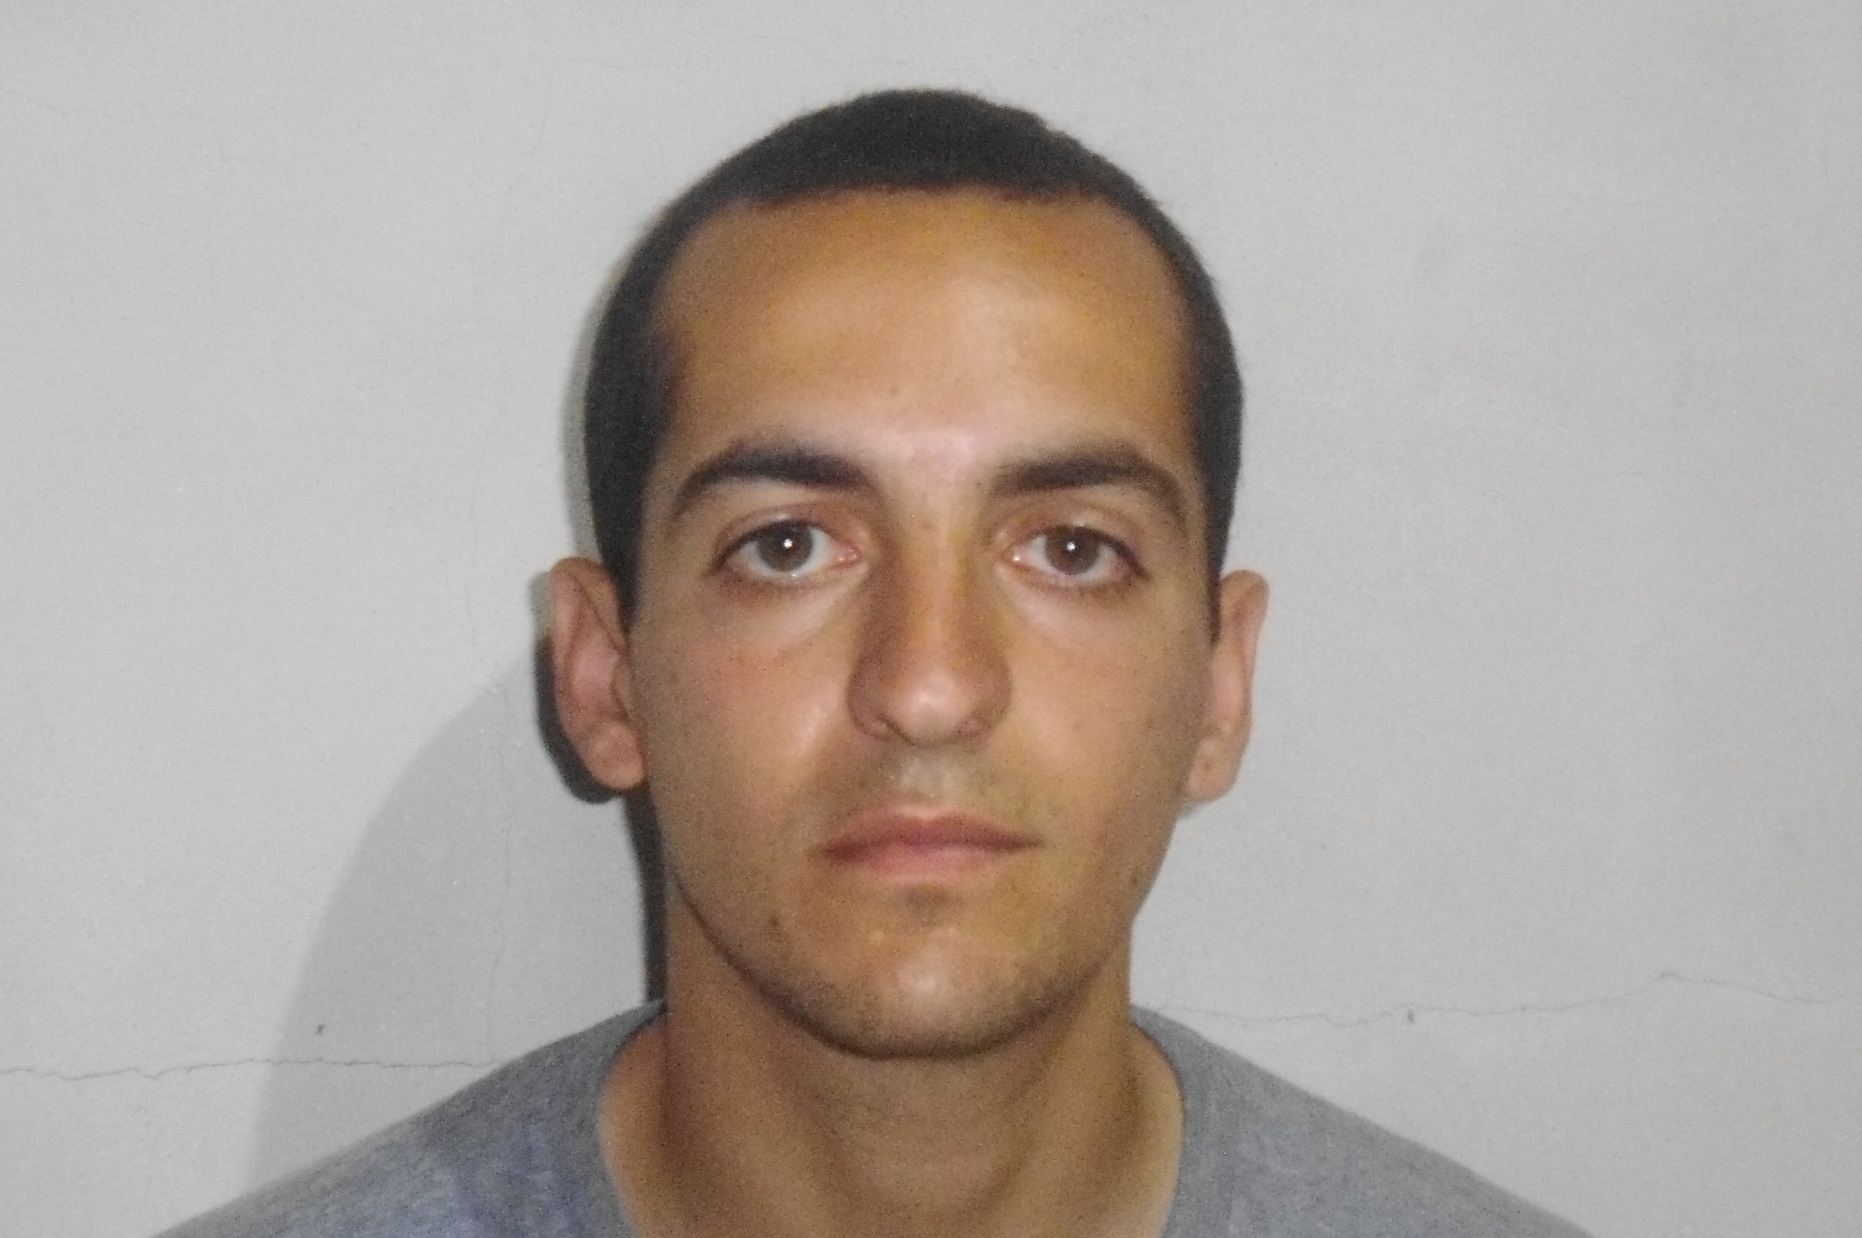
\includegraphics[width=4cm,clip=true,trim=7.5cm 0 7.5cm 0]{face}}
\end{picture}
\subsection*{Formación académica}
\subsubsection*{Secundario}
\normalsize{2006-2008. Modalidad economía y gestión.}\\\small{Colegio Sagrado Corazón, Venado Tuerto.}
\subsubsection*{Terciario}
\normalsize{2009-2011, 2015-2016. Analista en computación administrativa.}\\\small{Instituto Católico de enseñanza superior (ICES), Venado Tuerto.}
\subsubsection*{Otros estudios}
\normalsize{2015. Curso: Seguridad de la información.}\\\small{Universidad Tecnológica Nacional (UTN).}
\subsubsection*{Estudios en curso}
\normalsize{2012-2013. Licenciatura en ciencias de la computación. Estado: 10 materias aprobadas.}\\
\small{Facultad de ciencias exactas, ingenieria y agrimensura (FCEIA), Rosario.}
\subsection*{Idiomas}
\begin{tabular}{l l}
  Inglés&Nivel medio\\
\end{tabular}
\subsection*{Experiencia laboral}
\begin{tabular}{l l}
  2014-Hoy&Cadetería Serpet\\
\end{tabular}
\subsection*{Otros datos de interés}
\begin{tabular}{l}
  Carné de conducir B-1\\
\end{tabular}
\end{document}